\documentclass{scrartcl}

\usepackage{graphicx}
\usepackage[utf8]{inputenc}
\usepackage[T1]{fontenc}
\usepackage{lmodern}
\usepackage[english]{babel}
\usepackage{amsmath}
\usepackage{amsthm}
\usepackage{mathtools}
\usepackage{amssymb}
\usepackage{listings}
\usepackage{xparse}
\usepackage{geometry}
\usepackage{enumerate}
\usepackage{tikz}
\usepackage{hyperref}
\usepackage[style=english]{csquotes}
\usepackage[language=english, backend=biber, style=alphabetic, sorting=nyt]{biblatex}

\hypersetup{
    colorlinks,
    linkcolor={red!50!black},
    citecolor={blue!50!black},
    urlcolor={blue!80!black}
}

\usetikzlibrary{babel, positioning, shapes.geometric, arrows, arrows.meta}
\addbibresource{bibliography.bib}

\title{Definition of Schemes}
\author{Simon Pohmann}

\newcommand{\N}{\mathbb{N}}
\newcommand{\Z}{\mathbb{Z}}
\newcommand{\F}{\mathbb{F}}
\newcommand{\I}{\mathbb{I}}
\newcommand{\V}{\mathbb{V}}
\newcommand{\C}{\mathbb{C}}
\newcommand{\p}{\mathfrak{p}}
\newcommand{\Set}{\mathrm{\textbf{Set}}}
\newcommand{\Aff}{\mathrm{\textbf{Aff}}}
\newcommand{\Sch}{\mathrm{\textbf{Sch}}}
\newcommand{\Ring}{\mathrm{\textbf{Ring}}}
\newcommand{\Ab}{\mathrm{\textbf{Ab}}}
\newcommand{\Mod}[1]{\text{\textbf{$#1$-Mod}}}
\newcommand{\Proj}{\mathbb{P}}
\newcommand{\im}{\mathrm{im}}
\newcommand{\Top}{\mathrm{Top}}
\newcommand{\Spec}{\mathrm{Spec}}
\newcommand{\Quot}{\mathrm{Quot}}
\renewcommand{\O}{\mathcal{O}}
\DeclareMathOperator*{\colim}{colim}

\newcommand\restr[2]{{
    \left.\kern-\nulldelimiterspace
    #1
    \vphantom{\big|}
    \right|_{#2}
}}

\newtheorem{prop}{Proposition}[section]
\newtheorem{theorem}[prop]{Theorem}
\newtheorem{lemma}[prop]{Lemma}
\newtheorem{corollary}[prop]{Corollary}

\theoremstyle{definition}
\newtheorem{problem}[prop]{Problem}
\newtheorem{alg}[prop]{Algorithm}
\newtheorem{definition}[prop]{Definition}
\newtheorem{example}[prop]{Example}
\newtheorem{remark}[prop]{Remark}

\begin{document}
\maketitle
\tableofcontents

\section{Category-theoretical stuff}
Let $\mathcal{C}$ be a sub-category of $\Set$ that has small limits and colimits, and let $X$ be a topological space.
\begin{definition}
    A \emph{sheaf} on $X$ is a functor
    \begin{equation*}
        F: \Top(X)^{\mathrm{op}} \to \mathcal{C}
    \end{equation*}
    that satisfies a local-to-global condition, i.e. for $(U_i)_i$ open and $s_i \in F(U_i)$ such that
    \begin{equation*}
        \restr{s_i}{U_i \cap U_j} = \restr{s_j}{U_i \cap U_j}
    \end{equation*}
    there exists a unique $s \in F(\bigcup_i U_i)$ such that
    \begin{equation*}
        \restr{s}{U_i} = s_i
    \end{equation*}
    Here we write $\restr{s}{V}$ for the image of $s \in F(U)$ under the map $F(U) \to F(V)$ (which we get from the inclusion morphism $V \subseteq U$ in $\Top(X)$).
\end{definition}
\begin{definition}
    Let $F$ be a sheaf on $X$. Then the \emph{stalk} of $F$ at some $x \in X$ is the colimit
    \begin{equation*}
        F_x := \colim_{U \ni x \ \text{open}} F(U)
    \end{equation*}
\end{definition}
\begin{prop}
    Let $F$ be a sheaf on $X$.
    Then for any open $U \subseteq X$ have that
    \begin{equation*}
        F(U) \cong \lim_{V \subseteq U \ \text{open}} F(V)
    \end{equation*}
\end{prop}
\begin{definition}
    Let $B$ be a basis of $X$.
    A $B$-sheaf is a functor
    \begin{equation*}
        F: \underbrace{\restr{\Top(X)}{B}^{\mathrm{op}}}_{\mathclap{\text{The subcategory of $\Top(X)$ containing only the objects from $B$}}} \to \mathcal{C}
    \end{equation*}
    that satisfies a local-to-global condition, i.e. for $(U_i)_i$ in $B$ and $s_i \in F(U_i)$ such that
    \begin{equation*}
        \forall x \in U_i \cap U_j \ \underbrace{\exists x \in V \subseteq U_i \cap U_j}_{\mathclap{\text{Since $B$ is a basis, there is always at least one such $V$}}}: \ \restr{s_i}{V} = \restr{s_j}{V} \quad \text{and} \quad U := \bigcup_i U_i \in B
    \end{equation*}
    there exists a unique $s \in F(U)$ such that
    \begin{equation*}
        \restr{s}{U_i} = s_i
    \end{equation*}
\end{definition}
\begin{theorem}
    \label{prop:extend_b_sheaves}
    Let $F$ be a $B$-sheaf for some basis $B$ of $X$.
    Then there exists a unique (up to unique isomorphism) sheaf $\tilde{F}$ on $X$ that extends $F$.
\end{theorem}
\begin{proof}
    First, we show Existence. For an open $U$ in $X$, define
    \begin{equation*}
        \tilde{F}(U) := \lim_{V \subseteq U, \ V \in B} F(V)
    \end{equation*}
    For an inclusion $U_1 \subseteq U_2$ and $s \in \tilde{F}(U_2)$, define then $\tilde{F}(U_1 \subseteq U_2)$ as the unique map such that
    \begin{equation*}
        \tilde{F}(U_2) \overset{\tilde{F}(U_1 \subseteq U_2)}{\to} \tilde{F}(U_1) \to F(V) \quad \text{is} \quad \tilde{F}(U_1) \to F(V)
    \end{equation*}
    for all $V \subseteq U_1, \ V \in B$.
    
    Now note that for $U_1 \subseteq U_2 \subseteq U_3$ we also have a map
    \begin{equation*}
        \tilde{F}(U_3) \to \tilde{F}(U_2) \to \tilde{F}(U_1)
    \end{equation*}
    that is compatible with the maps $F(V_1 \subseteq V_2)$ for $V_1 \subseteq V_2, \ V_1, V_2 \in B$, and so by uniqueness above, we see
    \begin{equation*}
        \tilde{F}(U_1 \subseteq U_3) = \tilde{F}(U_1 \subseteq U_2) \circ \tilde{F}(U_2 \subseteq U_3)
    \end{equation*}
    Furthermore, clearly $\tilde{F}(\mathrm{id}_U) = \mathrm{id}_{\tilde{F}(U)}$, so $\tilde{F}$ is a presheaf.
    Note that $\tilde{F}(V) \cong F(V)$ for all $V \in B$ and similar for morphisms, so indeed $\tilde{F}$ extends $F$.

    Now we show the local-to-global condition.
    Assume we have $(U_i)_i$ open in $X$ and $s_i \in \tilde{F}(U_i)$ such that
    \begin{equation*}
        \restr{s_i}{U_i \cap U_j} = \restr{s_j}{U_i \cap U_j}
    \end{equation*}
    Let $U = \bigcup_i U_i$. 
    By the local-to-global condition of $F$, for each $ V \subseteq U, \ V \in B$ there exists a unique $s_V \in \tilde{F}(V) = F(V)$ with
    \begin{equation*}
        \restr{s_V}{V_i} = \restr{s_i}{V_i} \quad \text{for all $V_i \subseteq U_i \cap V, \ V_i \in B$}
    \end{equation*}
    Since
    \begin{equation*}
        \lim_{V \subseteq U, \ V \in B} F(V) \cong \bigl\{ (a_V)_V \in \prod_V F(V) \bigm| F(V_1 \subseteq V_2)(a_{V_2}) = a_{V_1} \bigr\}
    \end{equation*}
    we see that these $s_V$ lift to one (necessarily unique) $s \in \tilde{F}(U)$.

    For Uniqueness, assume we have two such sheaves, say $G$ and $H$.
    Now note that for all open $U$ in $X$ with $V_i \in B$, we have
    \begin{equation*}
        G(U) \cong \bigl\{ (a_V)_V \in \prod_{V \subseteq U, \ V \in B} F(V) \bigm| F(V_1 \subseteq V_2)(a_{V_2}) = a_{V_1} \bigr\}
    \end{equation*}
    where $\supseteq$ follows from general structure and $\subseteq$ from the local-to-global property.
    The same holds for $H$, so $G \cong H$.
\end{proof}

\section{Schemes}
\begin{definition}
    A \emph{locally ringed space} is a topological space $X$ with a sheaf of rings $\O_X$ on $X$ such that all stalks $\O_{X, x}$ are local rings.
\end{definition}
\begin{definition}
    Let $R$ be a ring (commutative, unital).
    Then let $\O_{\Spec R}$ be the sheaf on $\Spec R$ that results from extending the B-sheaf
    \begin{equation*}
        \O_{\Spec R}(D_f) := R_f, \quad f \in R
    \end{equation*}
    to a sheaf as in Theorem~\ref{prop:extend_b_sheaves}.
    Here the sets
    \begin{equation*}
        D_f = \{ \mathfrak{p} \leq R \ | \ f \notin \mathfrak{p} \} \subseteq \Spec R
    \end{equation*}
    are the basic open sets and form a basis of $\Spec R$.
\end{definition}
\begin{definition}
    A \emph{morphism} between locally ringed spaces $(X, \O_X)$ and $(Y, \O_Y)$ is a continuous map $f: X \to Y$ together with a natural transformation $\eta: \O_Y \Rightarrow f_*\O_X$ that satisfies
    \begin{equation*}
        \eta_y: (f_*\O_X)_y \cong \O_{X, f(y)} \to \O_{Y, y} \quad \text{maps} \quad \eta_y(\mathfrak{m}) \subseteq \mathfrak{m}
    \end{equation*}
    for all $y \in Y$.
    We write $f$ for the morphism of schemes $(X, \O_X) \to (Y, \O_Y)$ and denote $\eta$ by $f^\# := \eta$.
    Here
    \begin{equation*}
        f_*: \mathrm{Sh}(X) \to \mathrm{Sh}(Y), \quad F \mapsto (U \mapsto F(f^{-1}(U)))
    \end{equation*}
    is the \emph{direct image functor} of the continuous map $f$.
\end{definition}
\begin{definition}
    Similar to the direct image functor, define for a continuous $f: X \to Y$ the \emph{inverse image functor} as the sheafification
    \begin{equation*}
        f^{-1}: \mathrm{Sh}(Y) \to \mathrm{Sh}(X), \quad F \mapsto \left( U \mapsto \colim_{V \supseteq f(U)} F(V) \right)^+
    \end{equation*}
\end{definition}
\begin{prop}
    $f^{-1} \dashv f_*$
\end{prop}
\begin{definition}
    A locally ringed space $(X, \O_X)$ is an \emph{affine scheme}, if there exists a ring $R$ such that $(X, \O_X) \cong (\Spec R, \O_{\Spec R})$.
\end{definition}
\begin{definition}
    A locally ringed space $(X, \O_X)$ is a \emph{scheme}, if there exists a covering $X = \bigcup_i U_i$ with open $U_i \subseteq X$ such that each $(U_i, \restr{\O_X}{U_i})$ is an affine scheme.
    Such $U$ are also called \emph{affine opens}.
\end{definition}
\begin{definition}
    Denote the category of schemes by $\Sch$ and the subcategory of affine schemes by $\Aff$
\end{definition}
\begin{definition}
    Let $\phi: R \to S$ be a ring homomorphism.
    Then this induces a morphism of affine schemes
    \begin{equation*}
        \Spec\phi: \Spec S \to \Spec R
    \end{equation*}
    given by
    \begin{equation*}
        \Spec\phi: \p \mapsto \phi^{-1}(\p)
    \end{equation*}
    and on basic open sets $D_g, \ g \in R$ by
    \begin{equation*}
        (\Spec\phi)_{D_g}: \O_{\Spec R}(D_g) \to \O_{\Spec S}(D_{\phi(g)}), \quad \frac x {g^k} \to \frac {\phi(x)} {\phi(g)^k}
    \end{equation*}
\end{definition}
\begin{prop}
    The functor
    \begin{equation*}
        \Spec: \Ring^{\mathrm{op}} \to \Aff
    \end{equation*}
    is an equivalence of categories.
\end{prop}
\begin{prop}
    Let $(X, \O_X)$ be a scheme. Then $X$ is T0.
\end{prop}
\begin{proof}
    Assume not, i.e. there are two points $x, y \in X$ such that every open neighborhood of $x$ contains $y$ and vice versa.
    As $(X, \O_X)$ has a cover by affine opens, consider an affine open $U$ containing $x, y$.
    Then $(U, \restr{\O_X}{U})$ is isomorphic to $\Spec R$ for some ring $R$.
    However, $\Spec R$ is T0, a contradiction. 
\end{proof}
\begin{definition}
    An open subscheme of a scheme $(X, \O_X)$ is $(U, \restr{\O_X}{U})$ for an open subset $U \subseteq X$.
\end{definition}
\begin{remark}
    The notion of a general subscheme is more tricky.
    We more or less want to have some subset $U \subseteq X$ and a corresponding sheaf $\O_U$ that should be derived from $\O_X$.
    However, we obviously cannot take $\restr{\O_X}{U}$, and in fact, it is not easy to find a suitable one.
    Hence, for now, we will remain with defining open subschemes. 
\end{remark}
\begin{definition}
    For a morphism of schemes $f: X \to Y$ and an open subscheme $U \subseteq X$ define the restriction as
    \begin{align*}
        &\restr{f}{U}: U \to Y, \quad x \in |U| \mapsto f(u), \\
        &\bigl(\restr{f}{U}\bigr)^\#_V: \O_Y(V) \to \O_X(f^{-1}(|V|) \cap U), \quad \alpha \mapsto \restr{f_V}{f^{-1}(|V|) \cap U}
    \end{align*}
\end{definition}

\section{Coproduct (gluing) in $\Sch$}

\begin{prop}
    For affine schemes $\Spec R_1$ and $\Spec R_2$ have that the coproduct in $\Sch$ is
    \begin{equation*}
        \Spec R_1 \sqcup \Spec R_2 = \Spec(R_1 \times R_2)
    \end{equation*}
\end{prop}
\begin{proof}
    Observe that
    \begin{equation*}
        \Spec(R_1 \times R_2) = \underbrace{\{ \p \times R_2 \ | \ \p \in \Spec R_1 \}}_{=: V_1} \cup \underbrace{\{ R_1 \times \p \ | \ \p \in \Spec R_2 \}}_{=: V_2}
    \end{equation*}
    First of all, the projection maps $\pi_i: R_1 \times R_2 \to R_i$ give rise to morphisms
    \begin{equation*}
        \phi_i: \Spec R_i \to \Spec(R_1 \times R_2)
    \end{equation*}
    So we have to show that this cocone is universal.

    Let $(W, \O_W)$ be a scheme with morphisms
    \begin{equation*}
        \psi_i: \Spec R_i \to (W, \O_W)
    \end{equation*}
    Define
    \begin{equation*}
        f: \Spec(R_1 \times R_2) \to W, \quad \begin{matrix*}
            \p \times R_2 &\mapsto\ \psi_1(\p) \\
            R_1 \times \p &\mapsto\ \psi_2(\p)
        \end{matrix*}
    \end{equation*}
    This is well-defined, as $\psi_i(R_i)$ is a point such that $\psi_i(\Spec R_i)$ is contained in every open neighborhood of it.
    Hence $\psi_1(R_1)$ and $\psi_2(R_2)$ cannot be separated by open sets, and thus must be equal as $W$ is T0.

    Furthermore, for any open $U \subseteq W$ note that
    \begin{equation*}
        f^{-1}(|U|) = \{ \p \times R_2 \ | \ \p \in \psi_1^{-1}(|U|) \} \cup \{ R_1 \times \p \ | \ \p \in \psi_2^{-1}(U) \}
    \end{equation*}
    is a union of open sets, hence open.
    So $f$ is continuous.

    Now note that
    \begin{equation*}
        (V_i, \restr{\O_{\Spec(R_1 \times R_2)}}{V_i}) \cong \Spec R_i
    \end{equation*}
    where the isomorphisms are natural in $V_i$.
    So $s \in \O_W(U)$ yields via $\O_W(U) \to \O_{\Spec R_i}(\psi^{-1}(|U|)) \cong \O_{\Spec(R_1 \times R_2)}(f^{-1}(|U|) \cap V_i)$ elements
    \begin{equation*}
        s'_1 \in \O_{\Spec(R_1 \times R_2)}(f^{-1}(|U|) \cap V_1), \quad s'_2 \in \O_{\Spec(R_1 \times R_2)}(f^{-1}(|U|) \cap V_2)
    \end{equation*}
    These glue together to some $s' \in \O_{\Spec(R_1 \times R_2)}(f^{-1}(|U|))$.
    Hence define a morphism of sheaves
    \begin{equation*}
        \eta: \O_W \to f_*\O_{\Spec(R_1 \times R_2)}, \quad \eta_U(s) := s'
    \end{equation*}
    as it is clearly compatible with restriction maps.

    Now, by construction, have that for $\p \in \Spec R_i$
    \begin{equation*}
        (f \circ \phi_i)(\p) = f(\pi_i^{-1}(\p)) = \psi_i(\p)
    \end{equation*}
    and
    \begin{equation*}
        \phi_i \circ \eta = \psi_i
    \end{equation*}
    The latter is true, as the isomorphism in
    \begin{equation*}
        \O_W(U) \to \O_{\Spec R_i}(\psi_i^{-1}(|U|)) \cong \O_{\Spec(R_1 \times R_2)}(f^{-1}(|U|) \cap V_i)
    \end{equation*}
    in the direction $\leftarrow$ on basic open sets is given by the extension of the projection map $\pi_i: (R_1 \times R_2)_g \to (R_i)_{\pi_i(g)}$ and hence is $\phi_i$.

    The uniqueness of the morphism $(f, \eta)$ is clear.
\end{proof}
\begin{prop}
    Let $(U_i)_i$ be a family of schemes with open subschemes $U_{ij} \subseteq U_i$ and isomorphisms $\phi_{ij}: U_{ij} \to U_{ji}$.
    If
    \begin{itemize}
        \item $U_{ii} = U_i$ and $\phi_{ii} = \mathrm{id}$
        \item $\phi_{ij}(U_{ij} \cap U_{ik}) \subseteq U_{ji} \cap U_{jk}$
        \item $\restr{\phi_{ik}}{U_{ij} \cap U_{ik}} = \phi_{jk} \circ \restr{\phi_{ij}}{U_{ij} \cap U_{ik}}$
    \end{itemize}
    then there is a scheme $X$ (unique up to unique isomorphism) with an open cover $X = \bigcup X_i$ and isomorphisms of schemes $\psi_i: U_i \to X_i$ such that
    \begin{equation*}
        \psi_j \circ \phi_{ij} = \restr{\psi_i}{U_{ij}}
    \end{equation*}
\end{prop}
\begin{remark}
    The above easily shows that coproducts exist in $\Sch$ (just take $U_i$ to be the empty scheme $(\emptyset, \emptyset \mapsto \{0\})$).
    However, $\Sch$ is not cocomplete\footnote{\href{https://mathoverflow.net/questions/9961/colimits-of-schemes}{https://mathoverflow.net/questions/9961/colimits-of-schemes}}, so coequalizers do not exist in general.
\end{remark}
\begin{prop}
    Let $X, Y$ be schemes and $X = \bigcup_i X_i$ a cover by open subschemes.
    Let further $f_i: X_i \to Y$ be morphisms such that for $i, j$ have
    \begin{equation*}
        \restr{f_i}{X_i \cap X_j} = \restr{f_j}{X_i \cap X_j}
    \end{equation*}
    Then there exists a unique morphism $f: X \to Y$ such that $\restr{f}{X_i} = f_i$.
\end{prop}

\section{Products in $\Sch$}

The fiber product allows us to define fibers in an abstract sense.
First, we show that preimages of open subschemes are open subschemes, i.e. have the natural scheme structure and behave as we would expect them to.
\begin{prop}[Preimages of open sets]
    Let $f: X \to Y$ be a morphism of schemes and let $U \subseteq Y$ be an open subscheme.
    Then the scheme $(f^{-1}(|U|), \restr{\O_X}{f^{-1}(|U|)})$ is the fiber product $X \times_Y U$.
\end{prop}
\begin{proof}
    Clearly, the open subscheme $Z := (f^{-1}(|U|), \restr{\O_X}{f^{-1}(|U|)})$ makes the diagram
    \begin{center}
        \begin{tikzpicture}
            \node (Z) at (0, 0) {$Z$};
            \node (X) at (-1.5, -1.5) {$X$};
            \node (U) at (1.5, -1.5) {$U$};
            \node (Y) at (0, -3) {$Y$};

            \draw [->] (Z) -- (X);
            \draw [->] (Z) -- (U) node [midway, right] {$f$};
            \draw [->] (X) -- (Y) node [midway, left] {$f$};
            \draw [->] (U) -- (Y);
        \end{tikzpicture}
    \end{center}
    commute.
    Hence, to show that it is the fiber product, we have to show universality.
    Assume $W$ is another scheme with compatible maps $g_x: W \to X$ and $g_u: W \to U$.
    Now define the morphism of schemes $h: W \to Z$ by
    \begin{align*}
        &h: |W| \to |U|, \quad w \in |W| \mapsto g_x(w) \\
        &h^\#_V: \O_Z(V) = \O_X(V) \to \O_W(g_x^{-1}(|V|)), \quad \alpha \mapsto (g_x)^\#_V(\alpha)
    \end{align*}
    This is well-defined, as for $w \in |W|$, have $f(g_x(w)) = g_u(w) \in U$ and so $w \in f^{-1}(|U|)$.
    Clearly, $f \circ h = g_u$ and $h = g_x$ up to restriction.
    The uniqueness of $h$ is clear as well. 
\end{proof}
From now on, use $f^{-1}(U)$ for the open subscheme $(f^{-1}(|U|), \restr{\O_X}{f^{-1}(|U|)}) = X \times_Y U$.
\begin{prop}
    Let $f: X \to Z$ and $g: Y \to Z$ be schemes over a scheme $Z$.
    The fiber product (or pullback) $X \times_Z Y$ is defined as the limit of
    \begin{equation*}
        X \overset{f}{\rightarrow} Z \overset{g}{\leftarrow} Y
    \end{equation*}
    (Finite) fiber products exist in $\Sch$.
\end{prop}
\begin{proof}
    We show that binary fiber products exist.
    Let $f: X \to Z, \ g: Y \to Z$ be as above.

    \paragraph{Step 1: $X, Y, Z$ affine} Assume $X = \Spec R, \ Y = \Spec S, \ Z = \Spec T$ and $f, g$ are induced by ring homomorphisms
    \begin{equation*}
        f^\#: T \to R, \quad g^\#: T \to S
    \end{equation*}
    We claim that $\Spec(R \otimes_T S)$ with 
    \begin{equation*}
        (\cdot \otimes 1)^\#: \Spec(R \otimes_T S) \to \Spec R, \quad (1 \otimes \cdot)^\#: \Spec(R \otimes_T S) \to \Spec S
    \end{equation*}
    works.
    For this, it suffices to show that $R \otimes_T S$ is the pushout (i.e. co-fiber product) of $R, S$ considered as $T$-algebras.
    This follows easily from the universal property of the tensor product.
    \paragraph{Step 2: $Y, Z$ affine} Assume $Y = \Spec S, \ Z = \Spec T$.
    Let $X = \bigcup X_i$ be a cover of $X$ by affine opens.
    We want to glue all $X_i \times_Z Y$.

    Note that $U_i := X_i \times_Z Y$ comes with a map $\pi_i: U_i \to X_i$.
    Now we can consider the open subscheme
    \begin{equation*}
        U_{ij} := \Bigl( \pi_i^{-1}(X_i \cap X_j), \ \restr{\O_{X}}{\pi_i^{-1}(X_i \cap X_j)} \Bigr)
    \end{equation*}
    Claim: $U_{ij}$ is the fiber product $(X_i \cap X_j) \times_Z Y$.
    Clearly $U_{ij}$ has maps $U_{ij} \to X_i \cap X_j$ and $U_{ij} \to Y$ inherited from $U_i \to X_i$ and $U_i \to Y$ such that
    \begin{center}
        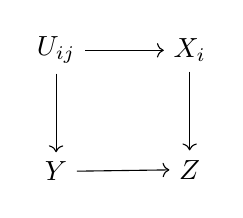
\begin{tikzpicture}
            \node (prod) {$U_{ij}$};
            \node [below = of prod] (Y) {$Y$};
            \node [right = of prod] (X) {$X_i$};
            \node [below = of X] (Z) {$Z$};
            \draw [->] (prod) -- (Y);
            \draw [->] (prod) -- (X);
            \draw [->] (X) -- (Z);
            \draw [->] (Y) -- (Z);
        \end{tikzpicture}
    \end{center}
    commutes.
    It is also not too hard to show that another scheme $W$ with compatible maps $W \to X_i \cap X_j$ and $W \to Y$ factors through $U_{ij}$.

    Hence, there is a unique isomorphism $\phi_{ij}: U_{ij} \to U_{ji}$ by the uniqueness of limits.
    Claim: The $U_i$, $U_{ij}$ and $\phi_{ij}$ satisfy the gluing conditions.
    \begin{itemize}
        \item Clearly $U_{ii} = U_i$ and so $\phi_{ii} = \mathrm{id}$ as there is a unique isomorphism $U_i \to U_i$.
        \item Note that by choice of $\phi_{ij}$ we know that the diagram
        \begin{center}
            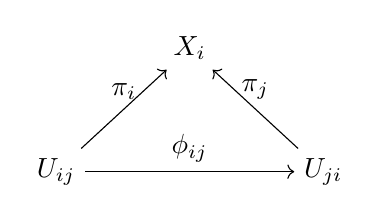
\begin{tikzpicture}
                \node (X) {$X_i$};
                \node [below left = of X] (Ui) {$U_{ij}$};
                \node [below right = of X] (Uj) {$U_{ji}$};
                \draw [->] (Ui) -- (X) node [midway, above] {$\pi_i$};
                \draw [->] (Uj) -- (X) node [midway, above] {$\pi_j$};
                \draw [->] (Ui) -- (Uj) node [midway, above] {$\phi_{ij}$};
            \end{tikzpicture}
        \end{center}
        is commutative.
        Hence $\phi_{ij}^{-1}(\pi_j^{-1}(X_i \cap X_j)) = \pi_i^{-1}(X_i \cap X_j)$ and so $\phi_{ij}^{-1}(U_{ij}) \subseteq U_{ji}$.
        \item Let
        \begin{equation*}
            U_{ijk} := \Bigl( \pi_i^{-1}(X_i \cap X_j \cap X_k), \ \restr{\O_{X}}{\pi_i^{-1}(X_i \cap X_j \cap X_k)} \Bigr) = U_{ij} \cap U_{ik}
        \end{equation*}
        A similar argument as above also shows that $U_{ijk}$ is the fiber product $(X_i \cap X_j \cap X_k) \times_Z Y$.
        Now, by uniqueness of limits, find that there is a unique isomorphism $U_{ijk} \to U_{kij}$.
        Note that both
        \begin{equation*}
            \restr{\phi_{ik}}{U_{ijk}} \quad \text{and} \quad \restr{\phi_{jk}}{U_{jik}} \circ \restr{\phi_{ij}}{U_{ijk}}
        \end{equation*}
        are such isomorphisms, hence 
        \begin{equation*}
            \restr{\phi_{ik}}{U_{ijk}} = \restr{\phi_{jk}}{U_{jik}} \circ \restr{\phi_{ij}}{U_{ijk}}
        \end{equation*}
    \end{itemize}
    Hence, we find a scheme $U$ that results from gluing all $X_i \times_Z Y$.
    Now we can glue all the morphisms $X_i \times_Z Y \to X_i$ and $X_i \times_Z Y \to Y$ to find compatible morphisms $U \to X$ and $U \to Y$.
    
    To show the universal property, assume there is a scheme $W$ with morphisms $W \to Z$.
    This induces morphisms $W \to X_i$ and $W \to Y$, hence we see that it factors as $W \to X_i \times_Z Y \to X \ \text{resp.} \ Y$.
    Gluing those maps $W \to X_i \times_Z Y$ then gives the expected map $W \to U$ and so $U$ is indeed the fiber product $X \times_Z Y$.

    \paragraph{Step 3: $Z$ affine} Exactly as in step 2 (note that we did not use $Y$ affine there).

    \paragraph{Step 4: General case} Let $Z = \bigcup Z_i$ be a cover of $Z$ by affine opens.
    Again, we would like to use Step 3 to construct parts as fiber products over $Z_i$ and glue them together.
    However, we cannot glue $X \times_{Z_i} Y$.
    Instead, let $X_i = f^{-1}(Z_i), Y_i = g^{-1}(Z_i)$ and glue
    \begin{equation*}
        X_i \times_{Z_i} Y_i = X_i \times_Z Y
    \end{equation*}
    First, we show this equality above.

\end{proof}

\section{Properties of Schemes and Morphisms}

\begin{prop}
    \label{prop:affine_local_property}
    Let $X$ be a scheme and let $P$ be a property of affine opens (i.e. a class of embeddings $\Spec R \to X$) such that
    \begin{itemize}
        \item for all $\alpha: \Spec R \to X$ and $f \in R$ have
        \begin{equation*}
           \text{$\alpha$ satisfies $P$} \quad \Rightarrow \quad \text{$\alpha_f$ satisfies $P$}
        \end{equation*}
        where $\alpha_f: \Spec R_f \to X$.
        \item for all $\alpha: \Spec R \to X$ and covers $\Spec R = \bigcup D_{f_i}$ have
        \begin{equation*}
            \text{all $\alpha_{f_i}$ satisfy $P$} \quad \Rightarrow \quad \text{$\alpha$ satisfies $P$}
        \end{equation*}
    \end{itemize}
    If there is a cover $X = \bigcup X_i$ of affine opens such that all inclusions $X_i \subseteq X$ satisfy $P$, then all inclusions $U \subseteq X$ of affine opens satisfy $P$.
\end{prop}

\begin{definition}
    A scheme $X$ is
    \begin{itemize}
        \item \emph{Noetherian}, if $|X|$ is quasi-compact and for all affine open $U$ have that $\O_X(U)$ is Noetherian.
        \item \emph{reduced}, if for all open $U$ have that $\O_X(U)$ is reduced.
        \item \emph{irreducible}, if $|X|$ is irreducible (i.e. not the union of two proper closed subsets).
        \item \emph{integral}, if for all open $U$ have that $\O_X(U)$ is integral.
    \end{itemize}
\end{definition}

Note that as defined before, the notion of an open subscheme is relatively easy.
Now we will also say what a closed subscheme is.

\begin{definition}
    Let $(X, \O_X)$ be a scheme.
    A scheme $(C, \O_C)$ is a closed subscheme of $(X, \O_X)$ if $C \subseteq X$ is closed and there exists a quasi-coherent sheaf of ideals $\mathcal{I}$ on $\O_X$ such that
    \begin{equation*}
        i_*\O_C \cong \O_X/\mathcal{I}
    \end{equation*}
    where $i: C \to X$ is the inclusion map and $i_*: \mathrm{Sh}(C) \to \mathrm{Sh}(X)$ its pullback.

    Here a sheaf of ideals $\mathcal{I}$ on $\O_X$ is called \emph{quasi-coherent}, if for all affine opens $U \subseteq X$, there exists an ideal $I \leq \O_X(U)$ such that
    \begin{equation*}
        \forall f \in \O_X(U): \ \mathcal{I}(D_f) = I \mathcal{O}_X(U)_f
    \end{equation*}
\end{definition}

\begin{definition}
    A morphism of schemes $f: X \to Y$ is
    \begin{itemize}
        \item \emph{affine}, if $f^{-1}(U)$ is affine for all affine open $U \subseteq X$.
        \item \emph{quasi-compact}, if $f^{-1}(U)$ is quasi-compact for all quasi-compact and open $U \subseteq X$.
        \item \emph{locally of finite type}, if for all affine opens $U \subseteq X$ and $V \subseteq Y$ with $f(U) \subseteq V$ have that $\O_X(U)$ becomes a finitely generated $\O_Y(V)$-algebra when equipped with 
        \begin{equation*}
            \O_Y(V) \ \overset{f^\#}{\to} \ \O_X(f^{-1}(V)) \ \to \ \O_X(U)
        \end{equation*}
        \item \emph{finite type}, if it is quasi-compact and locally of finite type
        \item a \emph{closed immersion}, if it is an isomorphism onto a closed subscheme of $Y$.
        \item an \emph{open immersion}, if it is an isomorphism onto an open subscheme of $Y$.
        \item \emph{flat}, if all $\O_{X, x}$ are flat $\O_{Y, f(x)}$-modules, i.e. the functor $\O_{X, x} \otimes_{\O_{Y, f(x)}} \cdot$ of $\O_{Y, f(x)}$-algebras is exact\footnote{here $\O_{X, x}$ becomes a $\O_{Y, f(x)}$-algebra via $f_x$}.
        \item \emph{separated}, if $\Delta: X \to X \times_B X$ is a closed immersion.
        Here $\Delta$ is the unique morphism $X \to X \times_B X$ such that $\pi_i \circ \Delta = \mathrm{id}_X$, where $\pi_i: X \times_B X \to X$.
        \item \emph{universally closed}, if for each $h: Z \to Y$ the unique morphism $X \times_Y Z \to Z$ that makes the diagram
        \begin{center}
            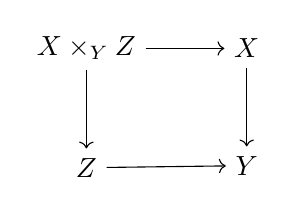
\begin{tikzpicture}
                \node (XZ) {$X \times_Y Z$};
                \node [right = of XZ] (X) {$X$};
                \node [below = of XZ] (Z) {$Z$};
                \node [below = of X] (Y) {$Y$};
                \draw [->] (XZ) -- (X);
                \draw [->] (XZ) -- (Z);
                \draw [->] (X) -- (Y);
                \draw [->] (Z) -- (Y);
            \end{tikzpicture}
        \end{center}
        commute is closed.
        \item \emph{proper}, if it is of finite type, separated and universally closed.
    \end{itemize}
    We say a scheme $X$ is separated, if the canonical morphism $X \to \Spec \Z$ is.
\end{definition}

\begin{definition}
    A scheme $X$ is called \emph{variety}, if it is of finite type, integral and separated.
\end{definition}

\begin{prop}[Characterization Noetherian]
    A quasi-compact scheme $X$ is Noetherian, if and only if there is a cover $X = \bigcup_i U_i$ of affine opens such that all $\O_X(U_i)$ are Noetherian.
\end{prop}

\begin{prop}[Characterization reduced]
    A scheme $X$ is reduced, if and only if all stalks $\O_{X, x}$ are reduced.
\end{prop}

\begin{prop}[Characterization irreducible]
    A scheme $X$ is irreducible, if and only if all affine opens $U \subseteq X$ are irreducible\footnote{Irreducibility is not affine-local, and it does not suffice to have a cover of irreducible affine opens.}. 
\end{prop}

\begin{prop}[Characterization integral]
    A scheme $X$ is integral, if and only if it is irreducible and reduced.
\end{prop}

\begin{prop}[Characterization flat]
    An $R$-module $M$ is flat if and only if for all injective $\alpha: N_1 \to N_2$ have that $\mathrm{id} \otimes \alpha: M \otimes_R N_1 \to M \otimes_R N_2$ is injective.
\end{prop}

\begin{prop}[Characterization closed immersion]
    For a morphism $f: X \to Y$ between schemes, the following are equivalent
    \begin{itemize}
        \item $f$ is a closed immersion
        \item $f: |X| \to f(|X|)$ is a homeomorphism and $f^\#: \O_Y \to f_*\O_X$ is surjective
        \item there exists a cover $Y = \bigcup_i U_i$ of affine opens and ideals $I_i \leq \O_Y(U_i)$ such that $f^{-1}(U_i) \cong \Spec(\O_Y(U_i)/I_i)$ as schemes over $U_i$.
        \item $f: |X| \to f(|X|)$ is a homeomorphism, $f(|X|)$ is closed and $f_*\O_X \cong \O_Y/\mathcal{I}$ for a quasi-coherent sheaf of ideals $\mathcal{I}$ on $\O_Y$
    \end{itemize}
\end{prop}
\begin{proof}
    First consider (i) $\Rightarrow$ (ii).
    Clearly $f: |X| \to f(|X|)$ is a homeomorphism.
    By assumption, have a sheaf of ideals $\mathcal{I}$ on $\O_Y$ such that $f_*\O_X \cong \O_Y/\mathcal{I}$ and $f: (|X|, \O_X) \to (f(|X|), \O_Y/\mathcal{Y})$ is an isomorphism.
    Now $f^\#$ factors as
    \begin{equation*}
        \O_Y \ \to \ \O_Y / \mathcal{I} \ \overset{\sim}{\to} \ \O_X
    \end{equation*}
    hence is surjective.

    To show (ii) $\Rightarrow$ (iii), let $Y = \bigcup_i U_i$ be a cover by affine opens.
    For each $i$, let now $I_i := \ker(f^\#_{U_i})$.
    As $f^\#$ is surjective, by the isomorphism theorem
    \begin{equation*}
        \tilde{f}^\#_{U_i}: \O_Y(U_i) / I_i \to (f_*\O_X)(U_i)
    \end{equation*}
    is an isomorphism of rings.
    Denote now $R = \O_Y(U_i)$ and consider a basic open set $D_g \subseteq U_i$.
    We have
    \begin{equation*}
        f^\#_{D_g}: R_g \to (f_*\O_X)(D_g)
    \end{equation*}
    is surjective and given by
    \begin{equation*}
        \frac {x} {g^n} \mapsto \frac {f^\#_{U_i}(x)} {f^\#_{U_i}(g)^n}
    \end{equation*}
    and thus has kernel $I_iR_g$.
    Hence, we see that also
    \begin{equation*}
        \tilde{f}^\#_{D_g}: R_g / I_i R_g \to (f_*\O_X)(D_g)
    \end{equation*}
    is an isomorphism.
    Hence, since the basic open sets form a basis, we see that there is an isomorphism of schemes
    \begin{equation*}
        \restr{\tilde{f}}{f^{-1}(U_i)}: f^{-1}(U_i) \to \Spec(R_g/I_iR_g)
    \end{equation*}
    which is also an isomorphism of schemes over $U_i$.
    This shows the claim.

    Finally, we show (iii) $ \Rightarrow$ (iv).
    Define a sheaf of ideals on $\O_Y$ by
    \begin{equation*}
        \mathcal{I}(U) := \bigcap_i \mathrm{restr}^{-1}_{U_i \cap U}(I_i)
    \end{equation*}
    Note that by assumption, each $\restr{\mathcal{I}}{U_i}$ is quasi-coherent.

    Claim: $\mathcal{I}$ is quasi-coherent.
    We show that ``$\restr{\mathcal{I}}{U}$ is quasi-coherent'' for affine opens $U \subseteq Y$ and the claim follows by Proposition~\ref{prop:affine_local_property}.
    \begin{itemize}
        \item If $\restr{\mathcal{I}}{U}$ is quasi-coherent with $U \cong \Spec R$, then clearly also $\restr{\mathcal{I}}{D_g}$ is where $g \in R$.
        This holds, as
        \begin{equation*}
            \mathcal{I}(D_g \cap D_h) = \mathcal{I}(D_{gh}) = \mathcal{I}(U) R_{gh}
        \end{equation*}
        \item Let $U = \bigcup_g D_g$ be a cover by basic open sets such that each $\restr{\mathcal{I}}{D_g}$ is quasi-coherent.
        Consider now a basic open set $D_h$ of $U$.
        By assumption, find for all $g$ that
        \begin{equation*}
            \mathcal{I}(D_g \cap D_h) = \mathcal{I}(D_{gh}) = \mathcal{I}(D_g) R_{gh}
        \end{equation*}
        where $R = \O_Y(U)$.
        By construction, have now that
        \begin{equation*}
            \mathcal{I}(D_h) = \bigcap_g \mathcal{I}(D_g)R_{gh}
        \end{equation*}
        The inclusion $\subseteq$ is clear.
        Since the $D_g$ cover $U$, we see that there is a combination $1 = \sum_i r_i g_i$ with $r_i \in R$.
        Now consider some $\alpha \in \bigcap_g \mathcal{I}(D_g) R_{gh}$.
        
        For each $g$ there is $n \in \N$ such that $\alpha h^n \in \mathcal{I}(D_g)$.
        Let now $N \in \N$ such that for all $i$, have $\alpha h^N \in \mathcal{I}(D_{g_i})$ (works as there are only finitely many such $i$).
        It follows that
        \begin{equation*}
            \restr{\alpha h^N}{D_{g_i} \cap D_{g_j}} = \restr{\alpha h^N}{D_{g_i} \cap D_{g_j}}
        \end{equation*}
        and so we can glue all $\alpha h^N$ to $\alpha h^N \in \mathcal{I}(U)$ by the sheaf property of $\mathcal{I}$.
        Thus $\alpha h^N \in \mathcal{I}(D_h)$ and so $\alpha \in \mathcal{I}(D_h)$.
    \end{itemize}
    Now it follows that for every affine open $U$ the restriction $\restr{\mathcal{I}}{U}$ is quasi-coherent, and so $\mathcal{I}$ is quasi-coherent.

    Claim: $f: (X, \O_X) \to (Y, \O_Y)$ is a closed immersion.
    Note that $f_* \O_X \cong \O_Y / \mathcal{I}$ as $\mathcal{I}(U) = \ker (\O_Y \to f_* \O_X)$ on each $U_i$ and so on each open $U$.
    Hence, it is left to show that $f(|X|)$ is closed.
    This follows directly, as the isomorphism $f^{-1}(U_i) \cong \Spec(\O_Y(U_i)/\mathcal{I}(U_i))$ is an isomorphism as schemes over $U_i$, and so the diagram
    \begin{center}
        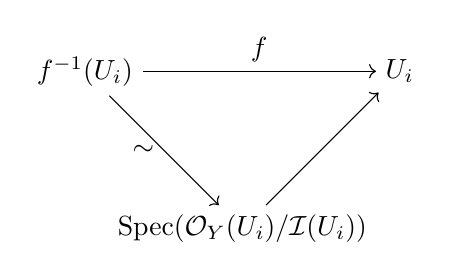
\begin{tikzpicture}
            \node (fUi) at (0, 0) {$f^{-1}(U_i)$};
            \node (Ui) at (4, 0) {$U_i$};
            \node (Spec) at (2, -2) {$\Spec(\O_Y(U_i)/\mathcal{I}(U_i))$};

            \draw [->] (fUi) -- (Ui) node [midway, above] {$f$};
            \draw [->] (fUi) -- (Spec) node [midway, left] {$\sim$};
            \draw [->] (Spec) -- (Ui);
        \end{tikzpicture}
    \end{center}
    is commutative, hence $\restr{f}{f^{-1}(U_i)}$ is a closed immersion, so $f(|f^{-1}(U_i)|)$ is closed in $|U_i|$.
    Furthermore, for a closed $C \subseteq f^{-1}(U_i)$ have that $f(C) \subseteq |U_i|$ is closed.
    Since the $U_i$ cover $Y$, we see that $f(|X|)$ is closed and $f: |X| \to f(|X|)$ is a homeomorphism.

    The last implication (iv) $\Rightarrow$ (i) follows directly from the fact that $f$ factors as
    \begin{equation*}
        (|X|, \O_X) \ \overset{\sim}{\to} \ (f(|X|), \O_{f(|X|)}) \ \overset{i}{\to} \ (|Y|, \O_Y)
    \end{equation*}
    where $i$ is the inclusion map and $\O_{f(|X|)}(U)$ is defined as $\O_Y(\tilde{U}) / \mathcal{I}(\tilde{U})$ where $\tilde{U} \subseteq Y$ is any open set with $\tilde{U} \cap f(|X|) = U$.
    In particular, we see that $i_*\O_{f(|X|)} \cong \O_Y/\mathcal{I}$ and so $(f(|X|), \O_{f(|X|)})$ is a closed subscheme.
\end{proof}

\section{Sheaves of modules}
Let $(X, \O_X)$ be a ringed space.
\begin{definition}
    A sheaf $F \in \Ab(X)$ such that each $F(U)$ is an $\O_X(U)$-module is called \emph{$\O_X$-module}, if for all $V \subseteq U$ open in $X$ have
    \begin{equation*}
        \restr{(\alpha x)}{V} = \restr{\alpha}{V} \cdot \restr{x}{V}
    \end{equation*}
    for all $\alpha \in \O_X(U)$ and $x \in F(U)$.
\end{definition}
Note that for $n \in \N$, the direct sum
\begin{equation*}
    \left( \bigoplus_{i = 0}^n \O_X \right)(U) := \bigoplus_{i = 0}^n \O_X(U)
\end{equation*}
is an $\O_X$-module.
Similarly, for any set $I$, the direct sum
\begin{equation*}
    \bigoplus_{i \in I} \O_X := \left( U \mapsto \bigoplus_{i \in I} \O_X(U) \right)^+
\end{equation*}
is an $\O_X$-module.
Note that we require the sheafification here.
\begin{definition}
    A morphism of $\O_X$-modules $F, G$ is a natural transformation $\eta: F \Leftarrow G$ such that each
    \begin{equation*}
        \eta_U: F(U) \to G(U)
    \end{equation*}
    is a $\O_X(U)$-module homomorphism.
\end{definition}
\begin{definition}
    For a morphism $f: F \to G$ of $\O_X$-modules define
    \begin{itemize}
        \item the \emph{kernel}
        \begin{equation*}
            \ker(f)(U) := \ker(f_U) \subseteq F(U)
        \end{equation*}
        which is a sub-$\O_X$-module of $F$.
        \item the \emph{cokernel}
        \begin{equation*}
            \mathrm{coker}(f) := \Bigl( U \mapsto G(U) / f_U(F(U)) \Bigr)^+
        \end{equation*}
        which is an $\O_X$-module.
        \item the \emph{image}
        \begin{equation*}
            \im(f) := \ker(G \to \mathrm{coker}(f)) = \Bigl( U \mapsto f_U(F(U)) \Bigr)^+
        \end{equation*}
        which is a sub-$\O_X$-module of $G$.
    \end{itemize}
    Call $f$ \emph{injective} if $\ker(f)$ is (everywhere) trivial and \emph{surjective} if $\im(f)$ is all of $G$, i.e. the canonical inclusion map $\im(f) \to G$ is an isomorphism.
\end{definition}
\begin{prop}
    $\ker$, $\mathrm{coker}$ and $\im$ are the kernel, cokernel and image respectively in the category theoretical sense.
\end{prop}
Note that a being a surjection $F \to G$ does not mean that $F(U) \to G(U)$ is surjective for all open $U$. 
\begin{definition}
    An $\O_X$-module $F$ is called
    \begin{itemize}
        \item \emph{generated by global sections}, if there exists a surjective morphism $\bigoplus_{i \in I} \O_X \to F$ for some set $I$
        \item \emph{locally generated by sections}, if each $x \in X$ has an open neighborhood $U$ such that $\restr{F}{U}$ is generated by global sections
        \item of \emph{finite type}, if each $x \in X$ has an open neighborhood $U$ such that there exists a surjection $\bigoplus_{i = 0}^n \O_U \to F$ for some $n \in \N$
        \item \emph{vector bundle} or \emph{locally free $\O_X$-module of finite rank}, if each $x \in X$ has an open neighborhood $U$ such that $\restr{F}{U} \cong \otimes_{i = 0}^n \O_U$ for some $n \in \N$
        \item \emph{line bundle} or \emph{invertible sheaf}, if each $x \in X$ has an open neighborhood $U$ such that $\restr{F}{U} \cong \O_U$.
        \item \emph{coherent}, if $F$ is of finite type and $\ker(f)$ is of finite type for all $n \in \N$, $U \subseteq X$ open and $f: \bigoplus_{i = 0}^n \O_U \to \restr{F}{U}$ homomorphism
        \item \emph{locally finitely presented}, if each $x \in X$ has an open neighborhood $U$ and $n, m \in \N$ as well as morphisms such that the sequence
        \begin{equation*}
            \bigoplus_{i = 0}^m \O_U \ \to \ \bigoplus_{i = 0}^n \O_U \ \to \ \restr{F}{U} \ \to \ 0
        \end{equation*}
        is exact\footnote{
            Note that an $R$-module $M$ is \emph{finitely presented}, if there exist $n, m \in \N$ and morphisms such that the sequence
            \begin{equation*}
                \bigoplus_{i = 0}^m R \ \to \ \bigoplus_{i = 0}^n R \ \to \ M \ to \ 0
            \end{equation*} 
            is exact.
            For a $k$-algebra $A$, we have such a sequence $k[y_1, ..., y_m] \to k[x_1, ..., x_n] \to A \to 0$ with $y_i \mapsto f_i$ iff $A \cong k[x_1, ..., x_n]/(f_1, ..., f_m)$.
        }
    \end{itemize}
\end{definition}
First, we consider two technical lemmas that describe under which conditions we can lift maps $\bigoplus_{i = 0}^n \O_{X, x} \to F_x$ to an open neighborhood of $x$.
\begin{lemma}
    Let $F$ be an $\O_X$-module of finite type and $x \in X$.
    Suppose there is $n \in \N$ and a surjection $\phi_x: \bigoplus_{i = 0}^n \O_{X, x} \to F_x$.
    Then there exists an open neighborhood $U$ of $x$ and a surjection $\phi: \bigoplus_{i = 0}^n \O_U \to \restr{F}{U}$ such that $\restr{\phi}{x} = \phi_x$.
\end{lemma}
\begin{lemma}
    Let $F$ be an $\O_X$-module of finite type and $x \in X$.
    Suppose there is $n \in \N$ and an isomorphism $\phi_x: \bigoplus_{i = 0}^n \O_{X, x} \to F_x$.
    If $\ker(f)$ is of finite type, then there exists an open neighborhood $U$ of $x$ and an isomorphism $\phi: \bigoplus_{i = 0}^n \O_U \to \restr{F}{U}$ such that $\restr{\phi}{x} = \phi_x$.
\end{lemma}
A corollary of these two technical lemmas is the following.
\begin{prop}
    Let $F$ be an $\O_X$-module.
    Suppose $F$ is coherent and for all $x \in X$, there is $n \in \N$ such that the stalk is free $F_x \cong \bigoplus_{i = 0}^n \O_{X, x}$.
    Then $F$ is a vector bundle.
\end{prop}
\begin{definition}
    For $\O_X$-modules $F, G$ and $(F_i)_{i \in I}$ define the
    \begin{itemize}
        \item \emph{coproduct} as
        \begin{equation*}
            \bigoplus_{i \in I} F_i := \left( U \mapsto \bigoplus_{i \in I} F_i(U) \right)^+
        \end{equation*}
        \item \emph{product} as
        \begin{equation*}
            \left( \prod_{i \in I} F_i \right)(U) := \prod_{i \in I} F_i(U)
        \end{equation*}
        \item \emph{tensor product} as
        \begin{equation*}
            F \otimes_{\O_X} G := \left( U \mapsto F(U) \otimes_{\O_X(U)} G(U) \right)^+
        \end{equation*}
    \end{itemize}
\end{definition}
\begin{prop}
    The product and coproduct defined above are product and coproduct in the category theoretical sense.
\end{prop}
\begin{definition}
    For a morphism $f: X \to Y$ of ringed spaces, an $\O_X$-module $F$ and an $\O_Y$-module $G$, define
    \begin{itemize}
        \item the \emph{direct image}
        \begin{equation*}
            (f_*F)(U) := F(f^{-1}(U))
        \end{equation*}
        which is an $f_*\O_X$-module, and thus an $\O_Y$-module.
        \item the \emph{inverse image}
        \begin{equation*}
            f^{-1}G := \left( U \mapsto \colim_{V \supseteq f(U)} G(V) \right)
        \end{equation*}
        which is an $f^{-1}\O_Y$-module.
        \item the \emph{pullback}
        \begin{equation*}
            f^*G := f^{-1}G \otimes_{f^{-1}\O_Y} \O_X
        \end{equation*}
        where $\O_X$ becomes an $f^{-1}\O_Y$-module via the unique morphism
        \begin{equation*}
            \colim_{V \supseteq f(U)} \O_X(V) \to \O_X(U)
        \end{equation*}
        given by the universal property of the colimit.
        This is an $f^{-1}\O_Y$-module and an $\O_X$-module (via $\alpha(x \otimes \beta) := x \otimes \alpha \beta$).
    \end{itemize}
\end{definition}
\begin{prop}
    For a morphism $f: X \to Y$ of ringed spaces have $f^* \dashv f_*$.
    Here
    \begin{align*}
        f_*: \Mod{\O_X} \to \Mod{\O_Y}, \quad F \mapsto f_*F \\
        f^*: \Mod{\O_Y} \to \Mod{\O_X}, \quad G \mapsto f^*G
    \end{align*}
    are the corresponding functors.
\end{prop}
\end{document}